\documentclass[titlepage = firstcover]{scrartcl}
\usepackage[aux]{rerunfilecheck}
\usepackage{fontspec}
\usepackage[main=ngerman, english, french]{babel}

% mehr Pakete hier
\usepackage{expl3}
\usepackage{xparse}

%Mathematik------------------------------------------------------
\usepackage{amsmath}   % unverzichtbare Mathe-Befehle
\usepackage{amssymb}   % viele Mathe-Symbole
\usepackage{mathtools} % Erweiterungen für amsmath
\usepackage[
  math-style=ISO,    % \
  bold-style=ISO,    % |
  sans-style=italic, % | ISO-Standard folgen
  nabla=upright,     % |
  partial=upright,   % /
]{unicode-math}% "Does exactly what it says on the tin."
\usepackage[section, below]{placeins}

% Laden von OTF-Mathefonts
% Ermöglich Unicode Eingabe von Zeichen: α statt \alpha

\setmathfont{Latin Modern Math}
%\setmathfont{Tex Gyre Pagella Math} % alternativ zu Latin Modern Math
\setmathfont{XITS Math}[range={scr, bfscr}]
\setmathfont{XITS Math}[range={cal, bfcal}, StylisticSet=1]

\AtBeginDocument{ % wird bei \begin{document}
  % werden sonst wieder von unicode-math überschrieben
  \RenewDocumentCommand \Re {} {\operatorname{Re}}
  \RenewDocumentCommand \Im {} {\operatorname{Im}}
}
\usepackage{mleftright}
\setlength{\delimitershortfall}{-1sp}

%Sprache----------------------------------------------------------
\usepackage{microtype}
\usepackage{xfrac}
\usepackage[autostyle]{csquotes}    % babel
\usepackage[unicode, pdfusetitle]{hyperref}
\usepackage{bookmark}
\usepackage[shortcuts]{extdash}
%Einstellungen hier, z.B. Fonts
\usepackage{booktabs} % Tabellen


\title{Wärmeleitfähigkeit}
\author{
  David Gutnikov\\
  \href{mailto:david.gutnikov@udo.edu}{david.gutnikov@udo.edu}
 \and 
  Lasse Sternemann\\
  \href{mailto:lasse.sternemann@udo.edu}{lasse.sternemann@udo.edu}
}
\date{Durchführung am 10.12.2019}


\begin{document}
  \maketitle
  \newpage
  \tableofcontents
  \newpage

  \section{Zielsetzung}
    Mithilfe dieses Versuch sollen die Wärmeleitfähigkeiten für verschiedene Materialien bestimmt werden.

  \section{Theoretische Grundlagen}
    Wärme kann innerhalb eines Körpers durch Konvektion, Wärmestrahlung oder Wärmeleitung transportiert werden.
    Dabei wird Wärmeleitung durch frei bewegliche Elektronen oder Gitterschwingungen, den Phononen, des Materials betrieben.
    In Metallen, welche in diesem Versuch betrachtet, werden geschieht dies haupsächlich durch die freien Elektronen.
    Damit Wärmeleitung stattfindet muss ein Temperaturgradient in dem Körper vorhanden sein.
    Es herrscht ein Temperaturgefälle von einem zum anderen Ende eines Stabes der Dichte $\rho$, der Länge $l$,
    der Querschnittsfläche $A$ und der spezifischen Wärmekapazität $c$ vor. Für die Wärmemenge $dQ$, die im Zeitraum $dt$
    durch $A$ fließt, gilt folgende Formel:
    \begin{equation}
      dQ = -\kappa A \frac{\partial T}{\partial x} \partial t = j_w A \partial t
    \end{equation}
    Wobei $\kappa$ die gesuchte Wärmeleitfähigkeit des Materials und $j_w$ die Wärmestromdichte ist.
    Mit Hilfe der Kontinuitätsgleichung \eqref{eqn:kontinuitätsgl} für lineare Wärmeströme,
    \begin{equation}
        \label{eqn:kontinuitätsgl}
      \frac{\partial T}{\partial t} + \frac{1}{\rho c} \frac{\partial j_w}{\partial x} = 0
    \end{equation}
    ergibt sich beim Einsetzen von $j_w$ die Wärmeleitungsgleichung \eqref{eqn:wärmeleitungsgl}:
    \begin{equation}
        \label{eqn:wärmeleitungsgl}
      \frac{\partial T}{\partial t} = \frac{\kappa}{\rho c} \frac{\partial^2 T}{\partial x^2}
    \end{equation}
    
    \noindent
    Werden lange Stäbe, um die es sich in diesem Versuch handelt, mit einer Periode $T_periode$ erhitzt und geküklt,
    so sieht die Lösung von \eqref{eqn:wärmeleitungsgl}, also die sich ergebende Temperaturwelle wie folgt aus:
    \begin{equation}
      T(x, t) = T_{\text{max}} e^{\sqrt{\frac{\omega \rho c}{2 \kappa}}x} \cos \biggl(\omega t - \sqrt{\frac{\omega \rho c}{2 \kappa}}x \biggr)
    \end{equation}
    \newpage

  \section{Versuchsdurchführung}
    Es werden vier Stäbe gleicher Maße, davon einer aus Aluminium, Edelstahl und zwei aus Messing, auf einer Platine \ref{fig:platine}
    eingespannt, sodass sie mithilfe eines Peltierelementes gleichzeitig an einem Ende erwärmt und gekühlt werden können.
    Es sind je zwei Thermoelemente zu Temperaturmessung in gleichem Abstand an den Stäben angebracht. Die Thermoelemente
    sind mit einem Gerät verbunden, welches die gemessenen Daten in bestimmten Zeitabständen aufnimmt. Die Stäbe müssen
    während den Messungen immer mit einer Wärmeisolierung bedeckt sein, damit die Werte nicht durch äußere Einflüsse
    verfälscht werden. Nach den Messungen soll die Wärmeisolierungentfernt werden, um die Stäbe wieder schneller 
    auf Zimmertemperatur runter zu kühlen.
    \subsection{Statische Methode}
      Hierbei werden die Stäbe so lange erwärmt bis Thermoelement 7 eine Temperatur von ca. 45° anzeigt. Die Spannung
      am Peltierelement beträgt 5V bei maximalem Strom und die Temperaturwerte an den Thermoelementen werden mit einer
      Abtastrate von 5 Sekunden abgenommen.
    \subsection{Dynamische Methode}
      Diese Messungen werden so lange ausgeführt bis eins der Thermoelemente 80° anzeigt, dabei beträgt die Spannung am
      Peltierelement 8V bei maximalem Strom. Bei der ersten Messreihe wird das Peltierelement mit einer Periode von
      80 Sekunden umgestellt, sodass die Stäbe abwechselnd erwärmt und gekühlt werden. Für die zweite Messreihe werden
      die Perioden auf 200 Sekunden verlängert. Dabei wird eine Abtastrate der Messwerte von 2 Sekunden genommen.
    
    \begin{figure}[h]
      \centering
      \label{fig:platine}
      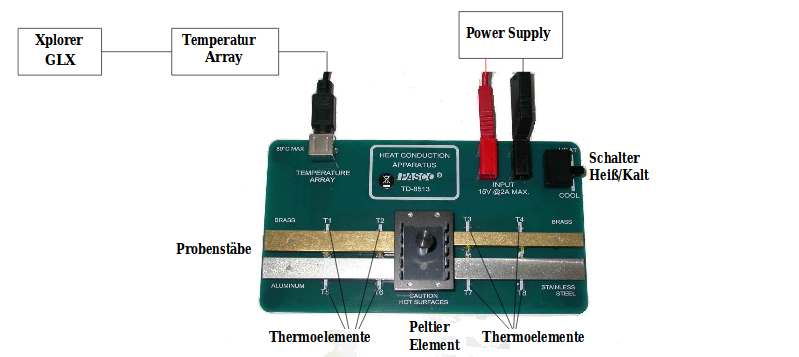
\includegraphics[width = 0.7\linewidth]{Platine.png}
    \end{figure}

    \FloatBarrier
\end{document}